\subsection{Sketchlet}
\label{sec:sketch}
The distributed sketch maintained by \textsc{Synopsis} is composed of many \emph{sketchlets} dispersed over a cluster of machines. Sketchlets maintain compact, multidimensional, tree-based representations of incoming data streams in the SIFT data structure. Each in-memory SIFT can be queried to retrieve statistical properties about the underlying data or discover how features interact. Due to the voluminous nature of these data streams, storing each individual record in main memory is not practical. Therefore, the queries supported by our framework are facilitated by compact, online metadata collection and quantization methods. These techniques ensure high accuracy while also conforming to the memory requirements of the system. To further improve accuracy, we bias our algorithms toward the most recent data points while reducing the resolution of the oldest.

\subsubsection{SIFT Structure}
\label{sec:sift}
SIFT instances are maintained as hierarchical trees with feature values stored in the vertices. Each level of the hierarchy, called a \emph{plane}, represents a particular data type, and traversing through vertices in this feature hierarchy reduces the search space of a query. Upon insertion of a multidimensional observation, each feature is arranged to form a \emph{path} through the tree and added based on the current feature hierarchy. Paths taken through the tree during a lookup are influenced by the specificity of the query, with additional feature expressions constraining the \emph{query scope}; an empty query would result in a scope that spans the entire tree. Figure~\ref{fig:sketch} demonstrates the structure of a tree within a SIFT and highlights a query and its scope. Note that any subset of the tree can be retrieved and manipulated in the same manner.

\begin{figure}[b!]
    \centerline{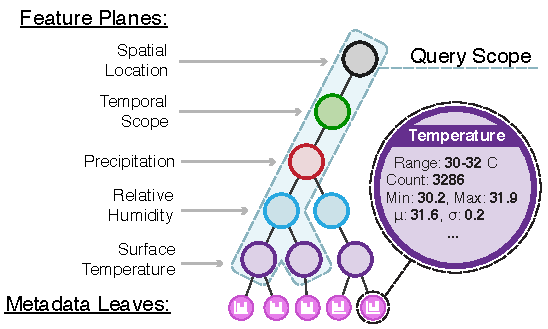
\includegraphics[width=3.2in]{figures/sketch.pdf}}
    \caption{A simplified SIFT tree with five planes and a sample query scope. In production settings, these trees contain hundreds of thousands of vertices and edges.}
    \label{fig:sketch}
\end{figure}

Metadata records for paths through the feature hierarchy are stored at leaf nodes. Each record contains statistics that are updated in an online fashion using Welford's~method~\cite{welford1962note}. Welford's method maintains the number of observations, $n$, the running mean, $\bar{x}$, and the sum of squares of differences from the current mean, $S_n$, as in the following recurrence relation:
\begin{align*}
    \bar{x}_0 &= 0, S_0 = 0 \\
    \bar{x}_n &= \bar{x}_{n - 1} + \frac{x_n - \bar{x}_{n - 1}}{n} \\
    S_n       &= S_{n - 1} + (x_n - \bar{x}_{n - 1})(x_n - \bar{x}_n)
\end{align*}
Besides the observation count and running mean, this enables calculation of the variance and standard deviation of the observed values:
\begin{align*}
    \sigma^2 = \frac{S_n}{n} \hspace{2em} \sigma = \sqrt{\frac{S_n}{n}}
\end{align*}
Our implementation of Welford's method also includes cross-feature relationships, such as the correlation between temperature values and humidity or the reflectivity of the earth and cloud cover. This is achieved by maintaining the sum of cross products between features. Leaf nodes may be \emph{merged} to combine their respective summary statistics into a single aggregate summary. This allows queries to be evaluated across multiple sketchlets and then fused into a single, coherent result.

\subsubsection{Structural Compaction}
The number of unique feature types stored in the SIFT directly influences the size of the hierarchy, impacting memory consumption. However, the number of vertices and edges that must be maintained by each tree can be managed by manipulating the hierarchical configuration. For instance, the memory impact of features that exhibit high variance over a large range can be mitigated by placing them toward the top of the hierarchy, while boolean features or those with low variance should be situated toward the bottom of the tree. Consequently, we \emph{compact} the logical representation of the SIFT by aggregating vertices from the entire forest and reorienting the planes to conserve memory. One notable result of this process is that vertices near the bottom of the hierarchy may be responsible for storing spatial locations of the data points rather than the root of the tree as depicted in our conceptual model of the SIFT; consider a dataset with sensor readings dispersed over fine-grained spatial areas. To allow efficient scaling in and out during tree migration to other sketchlets, full-resolution geohashes are stored in the hierarchy. If these hashes are maintained near the root of the tree, each spatial region will effectively be allocated its own unique portion of the SIFT. 

SIFT planes are reconfigured dynamically to achieve structural compaction based on their corresponding vertex \emph{fan-out} during the initial population of the trees. Boolean values or unique data points, such as a spatial location where a sensor resides, are moved toward the bottom of the tree. Using the observed ranges for each feature, a \emph{fan-out score} is calculated to determine the worst case impact of feature fan-out. Features with fan-out scores nearest to the overall mean score are pushed to the top of the hierarchy. This helps keep the trees as compact as possible near the root, with most expansion occurring near the leaves, leading to increased path similarity.  During this phase, full-resolution feature values are stored at each vertex, but once a steady state is reached the \emph{quantization} process begins to determine bin sizes and further compact the planes.

\subsubsection{Density-Driven Quantization}
Maintaining data points, statistics, and cross-feature relationships in memory at full resolution is infeasible when faced with voluminous datasets, even when load is balanced over several computing resources. To reduce the memory consumption of SIFT instances we perform \emph{quantization} --- targeted reduction of resolution --- which allows vertices in the tree to be merged, thus enabling single vertices to represent a collection of values. We determine which vertices should be merged by splitting each range of feature values into a configurable number of \emph{bins}. After quantization, each vertex represents a range of observations.

To determine the size and quantity of these bins, trees within the SIFT maintain additional metadata provided by the multivariate online kernel density estimation (oKDE) algorithm developed by Kristan et al. \cite{kristan2011multivariate}. While it is possible to recompute kernel density estimates periodically for each feature type using in-memory samples \cite{malensek2013autonomously}, the online approach afforded by oKDE requires less overall CPU usage and memory, which is crucial in streaming environments.  oKDE assimilates data incrementally at runtime to create a dynamic probability density function (PDF) for each feature type. The smoothing parameter used to create the PDF, called the \emph{bandwidth}, is selected autonomously using Silverman's rule \cite{silverman1986density}. Silverman's rule assumes that data tends to follow a normal distribution, which is generally true for naturally-occurring observations. However, we also allow the smoothing parameter be selectively reconfigured for different problem types. During the quantization process, these PDFs are used to ensure that each bin is assigned an approximately equal proportion of the feature density, while the overall number of bins is influenced by memory availability. As a result, the majority of values for a given feature type will be stored in small, highly-accurate bins.

Figure~\ref{fig:quantization} illustrates the quantization process for the \emph{surface temperature} feature in our atmospheric test dataset \cite{noaa_nam}: the highest densities of values are stored in the smallest bins (indicated by vertical lines under the curve), improving overall accuracy. To evaluate accuracy, we compare the mean values of each bin with the actual, full-resolution data points. Consequently, the \emph{standard error} ($\sigma_{\bar{x}}$) can be calculated from our running summary statistics to judge the accuracy level of the bins based on how well they are represented by the mean:
\begin{align*}
    \sigma_{\bar{x}} = \sqrt{\frac{S_n}{n^2}}
\end{align*}
This information is provided alongside any query results returned by the system. During initialization, we calculate the normalized error for each data point empirically (shown in the lower portion of Figure~\ref{fig:quantization}). For values that are observed less frequently, the error rate is higher; temperatures from 240 -- 260 Kelvin (-33.15 to -13.15 \degree C) reach a normalized root-mean-square error (NRMSE) of about 7\%. However, approximately 80\% of the values in the tree will be assigned to vertices with an error of about 0.5\%. In practice, this means that commonly-observed values returned by \textsc{Synopsis} will be within 0.25 Kelvin of their actual value.
%
\begin{figure}
    \centerline{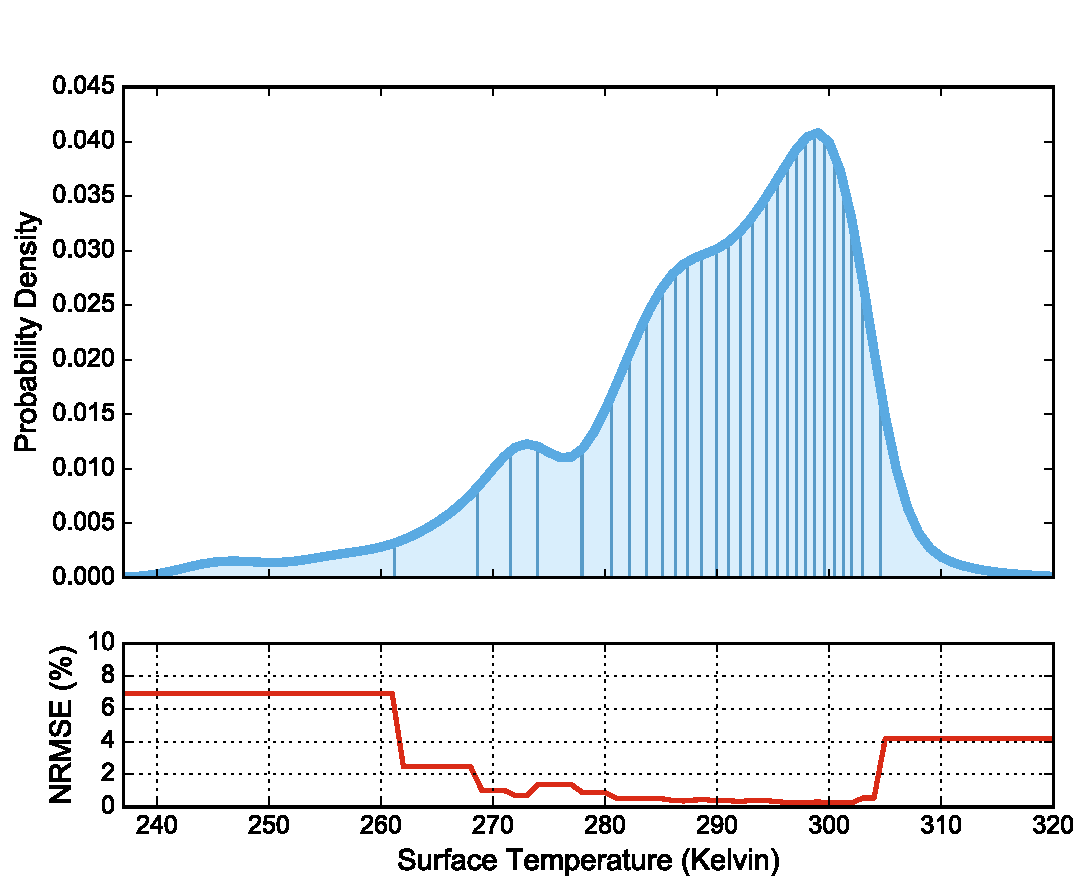
\includegraphics[width=3.5in]{figures/quantization.pdf}}
    \caption{A demonstration of the quantization process, with 29 vertex bins generated across the distribution of surface temperature values in our dataset. Each bin is indicated by a vertical line under the curve.}
    \label{fig:quantization}
\end{figure}
%
Table~\ref{tbl:tree-stats} compares full-resolution and quantized trees that were generated from a month of data with 20 unique features from our test dataset, which includes atmospheric information such as temperature, humidity, precipitation, and cloud cover. In this configuration, our autonomous quantization algorithm reduced memory consumption by about 62.4\%, which allows much more historical data to be maintained in each SIFT. Decreasing the memory footprint of the SIFT also allows larger geographical areas to be maintained by a single sketchlet.
%
\begin{table}[h!]
    \renewcommand{\arraystretch}{1.2}
    \caption{Tree statistics before and after our dynamic quantization algorithm over one month of ingested data.\vspace{-1em}}
    \label{tbl:tree-stats}
    \begin{center}
        \begin{tabular}{|l|c|c|c|}
            \hline
            \textbf{Metric} & \textbf{Original} & \textbf{Quantized} & \textbf{Change} \\
            \hline
            Vertices & 3,104,874 & 1,238,424 & -60.1\% \\
            \hline
            Edges    & 3,367,665 & 1,441,639 & -57.2\% \\
            \hline
            Leaves   & 262,792   & 203,216   & -22.7\% \\
            \hline
            Memory   & 1,710.6 MB & 643.1 MB  & -62.4\% \\
            \hline
        \end{tabular}
    \end{center}
\end{table}

\subsubsection{Temporal Dimensionality Reduction}
While our quantization approach enables \textsc{Synopsis} to retain large volumes of data in main memory, we also offer a temporal \emph{accuracy gradient} to ensure the most relevant data points are prioritized for high accuracy. This is achieved by iteratively removing tree paths from the SIFT hierarchy in the oldest subtrees, eventually phasing out old records. As data ages, this process results in the creation of temporal accuracy bands.

Selective temporal dimensionality reduction proceeds in a bottom-up fashion, starting from the bottom of the hierarchy. Given a set of relevant vertices, neighboring bins are merged uniformly across the feature space. As the bins are merged, their respective metadata is also merged, reducing memory consumption. Given two metadata instances, merging results in half the memory footprint. However, it is worth noting that this process is irreversible; once metadata has been merged, it cannot be split at a later point in time. As time passes, entire portions of the feature space are compacted until a single metadata record is left for a particular temporal range. This allows users to still query the summary statistics and models for historical data, but at a lower level of accuracy.
